El \textbf{encaminamiento en redes de conmutación de paquetes} es la función encargada de encontrar una ruta a través de la red entre pares de nodos finales para que la comunicación sea eficiente. A diferencia de la conmutación de circuitos, los datos se dividen en pequeñas unidades llamadas \textbf{paquetes}

Se denominan \textbf{paquetes} porque la información no fluye como un torrente continuo, sino que \textbf{se segmenta en bloques de longitud limitada} que contienen tanto datos de usuario como información de control (cabecera). El hecho de que sean paquetes implica una \textbf{arquitectura de almacenamiento y retransmisión (store-and-forward)}: cada paquete se recibe completamente en un nodo, se almacena brevemente y luego se transmite al siguiente.

\subsection{Requisitos de función de encaminamiento}

La función principal de una red de conmutación de paquetes es \textbf{aceptar paquetes procedentes de una estación emisora y enviarlos hacia una estación destino}. Para ello se debe determinar una ruta a través de la red, siendo posible la existencia de más de una. Se debe realizar una \textbf{función de encaminamiento}. Para ser efectivo, debe cumplir con varios criterios: \textbf{exactitud, simplicidad, robustez, estabilidad, imparcialidad, optimización y eficiencia}.

La \textbf{robustez} está relacionada con la habilidad de la red para enviar paquetes de alguna forma ante la aparición de sobre cargas y fallos localizados. La red puede reaccionar sin sufrir pérdidas de paquetes o caída de circuitos virtuales. La robustez puede implicar cierta inestabilidad. Las técnicas que reaccionan ante condiciones cambiantes presentan una tendencia no deseable a reaccionar lentamente ante determinados eventos o experimentar oscilaciones inestables de una situación extrema a otra. Es vital que el sistema reaccione ante fallos o congestión (robustez), pero sin generar oscilaciones inestables donde el tráfico rebote entre nodos (estabilidad).

Una técnica de encaminamiento implica cierto coste de procesamiento en cada nodo y, en ocasiones, también un coste en la transmisión, impidiéndose en ambos casos el funcionamiento eficiente de la red. 

\subsection{Elementos de diseño}

Con estos requisitos en mente vamos a evaluar los distintos elementos de diseño involucrados en un esquema de encaminamiento.

\subsubsection{Criterios de rendimiento}

La elección de una ruta se fundamenta generalmente en algún criterio de rendimiento. El más simple consiste en elegir el camino con menor número de saltos (aquel que atraviesa el menor número de nodos) a través de la red. Una generalización del criterio de menor número de saltos lo constituye el encaminamiento de mínimo coste. En este caso se asocia un coste a cada enlace y, para cualesquiera dos estaciones conectadas, se elige aquella ruta a través de la red que implique el coste total mínimo. La asignación de los costes a los enlaces se hace en función de los objetivos de diseño; por ejemplo, el coste podría estar inversamente relacionado con la velocidad (es decir, a mayor velocidad menor coste) o con el retardo actual de la cola asociada al enlace.

\begin{figure}[H]
	\centering
	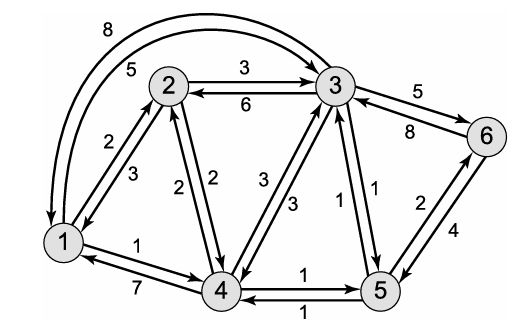
\includegraphics[width=0.5\textwidth]{img/conPaqueteEj1.png}
	\caption{Ejemplo de red de conmutación de paquetes}
	\label{fig:grafico3}
\end{figure}

\subsubsection{Instante y lugar de decisión}

Las decisiones de encaminamiento se realizan de acuerdo a criterio de rendimiento. Dos cuestiones importantes son el \textbf{instante temporal y el lugar en que se toma la decisión}.

El \textbf{instante de decisión} esta determinado por el hecho de que la decisión de encaminamiento se hace en base a un \textbf{paquete o a un circuito virtual}. Cuando la operación interna de la red se basa en datagramas, \textbf{la decisión de encaminamiento se toma de forma individual para cada paquete}. En el caso de circuitos virtuales internos, \textbf{la decisión sólo se realiza en el momento en que se establece un circuito virtual} ya que los demás paquetes siguen la misma ruta.

El \textbf{lugar de decisión} hace referencia al nodo/s en la red responsables de la decisión de encaminamiento. El más común es el \textbf{encaminamiento distribuido}, cada nodo de la red tiene la responsabilidad de seleccionar un enlace de salida sobre el que llevar a cabo el envío de los paquetes a medida que éstos se reciben. En \textbf{encaminamiento centralizado}, la decisión se toma por parte de algún nodo designado al respecto. Una tercera opción es \textbf{encaminamiento desde el origen}, es la estación origen quien toma la decisión de encaminamiento, comunicándosela a la red.

El instante y el lugar de decisión son variables de diseño independientes. En una red de datagramas, el paquete siguiente puede seguir una ruta diferente, determinada por cada nodo a lo largo del camino. En una red de circuitos virtuales, cada nodo recuerda la decisión de encaminamiento tomada cuando se estableció el circuito virtual, se limita a transmitir los paquetes sin tomar decisiones nuevas.

\subsubsection{Fuente de información de la red y tiempo de actualización}

La mayoría de los esquemas de encaminamiento requieren que las decisiones se tomen en base al conocimiento de la tipología de la red, carga y coste de los enlaces. Algunas estrategias, no hacen uso de ninguna información para la transmisión de los paquetes.

En el encaminamiento distribuido, cada uno de los nodos hacen uso de información local, como el coste asociado a los distintos enlaces de salida; e información de los nodos directamente conectados, como la congestión que experimentan ellos.

Finalmente, existen algoritmos de uso común que permiten al nodo obtener información de todos los nodos de una potencial ruta de interés. En encaminamiento centralizado, el nodo central hace uso generalmente de información procedente de todos los nodos.

El \textbf{tiempo de actualización de la información}, es función de la fuente de información y de la estrategia de encaminamiento. Si no se usa información no existe actualización. Si sólo se utiliza información local, la actualización es continua, porque un nodo individual conoce siempre sus condiciones locales actuales. Para el resto de categorías de fuentes de información el tiempo de actualización depende de la estrategia de encaminamiento. Para  encaminamiento estático, la información no se actualiza nunca, para una técnica adaptable la actualización se lleva a cabo periódicamente a fin de posibilitar la adaptación de la decisión de encaminamiento.

Cuanto mayor sea la información disponible y más frecuentemente se actualice ésta, más probable será que las decisiones de encaminamiento tomadas por la red sean buenas. Teniendo presente que la transmisión de esta información consume recursos de la red.

\subsection{Estrategias de encaminamiento}

Existen numerosas estrategias de encaminamiento para abordar las necesidades de encaminamiento en redes de conmutación de paquetes.

\subsubsection{Encaminamiento Estático}

Se configura una única ruta permanente para cada par de nodos \textbf{origen-destino} en la red, pudiéndose utilizar para ello cualquiera de los algoritmos de mínimo coste. Las rutas son fijas de modo que los costes de enlace usados para el diseño de las rutas no pueden estar basados en variables dinámicas como el tráfico.

Se crea una matriz de encaminamiento central, almacenada en un centro de control de red. Esta matriz especifica que para cada par de nodos origen-destino, la identidad del siguiente nodo en la ruta. Es suficiente conocer, para cada par, cuál es el primer nodo en la ruta. En cada punto a lo largo del camino sólo es necesario conocer la identidad del nodo siguiente, no la ruta completa.

A partir de esta matriz se pueden crear y almacenar en cada nodo las tablas de encaminamiento asociadas. Cada nodo sólo necesitará almacenar una columna de la tabla de encaminamiento, indicándose en ella el nodo siguiente para cada destino.

No existe diferencia entre datagramas y circuitos virtuales, ya que todos los paquetes que llegan con un destino concreto siguen la misma ruta. La ventaja es su simplicidad, además de su buen funcionamiento en redes fiables con carga estacionaria. Su desventaja radica en la falta de flexibilidad, ya que no reacciona ante fallos ni ante congestión en la red.
 
\begin{figure}[H]
	\centering
	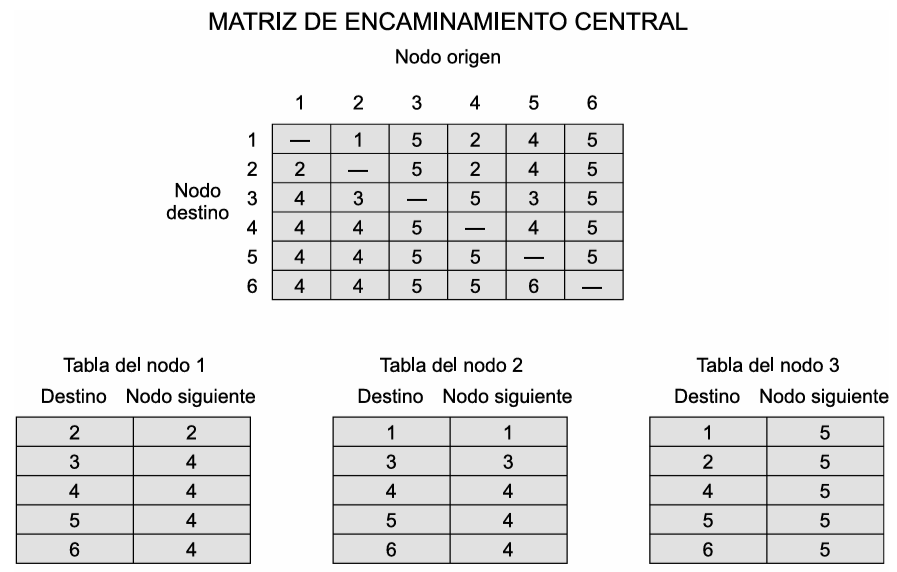
\includegraphics[width=0.5\textwidth]{img/matrizEncaminamiento.png}
	\caption{Matriz de Encaminamiento central}
	\label{fig:grafico4}
\end{figure}

\subsubsection{Inundaciones}

Otra técnica es la de inundaciones, la cual no precisa de ninguna información sobre la red. Un nodo origen envía un paquete a todos sus nodos vecinos, los cuales, a su vez, lo transmiten sobre todos los enlaces de salida excepto por el que llegó.

Una forma de prevenir estas retransmisiones consiste en incluir un campo de cuenta de saltos en cada paquete. Este contador puede ponerse inicialmente a un valor máximo, como es por ejemplo el diámetro de la red (TTL). Cada vez que un nodo transmite un paquete, decrementa la cuenta en uno, de modo que cuando el contador alcanza el valor cero se elimina el paquete de la red.

\begin{figure}[H]
	\centering
	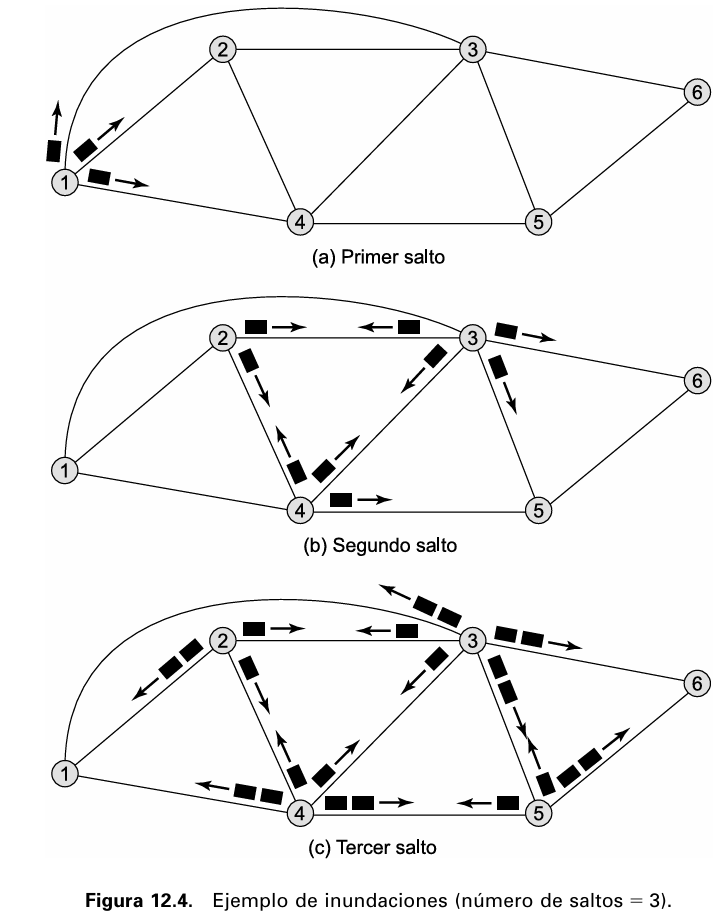
\includegraphics[width=0.5\textwidth]{img/inundacion.png}
	\caption{Matriz de Encaminamiento central}
	\label{fig:grafico5}
\end{figure}

La técnica de inundaciones presenta tres propiedades importantes:

\begin{itemize}
	\item Se prueban todos los posibles caminos entre los nodos origen y destino. Se garantiza la recepción del paquete siempre que exista, al menos, una ruta entre el origen y el destino.
	\item  Al menos una copia del paquete a recibir en el destino habrá usado una ruta de menor número de saltos.
	\item Se visitan todos los nodos que están directa o indirectamente conectados al nodo origen.
\end{itemize}

\subsubsection{Encaminamiento Aleatorio}

La técnica de encaminamiento aleatorio presenta, con menor tráfico, la sencillez y robustez de la técnica de inundaciones. En este esquema, un nodo selecciona un único camino de salida para retransmitir un paquete entrante; el enlace de salida se elige de forma aleatoria, excluyendo el enlace por el que llegó el paquete. Si todos los enlaces son igualmente probables de ser elegidos, una implementación sencilla consistiría en seleccionarlos de forma alternada.

Una mejora a esta técnica consiste en asignar una probabilidad a cada uno de los enlaces de salida y llevar a cabo la selección de acuerdo con estas probabilidades.

\subsubsection{Encaminamiento Adaptable}

En todas las redes de conmutación de paquetes se utiliza algún tipo de técnica de encaminamiento adaptable; las decisiones de encaminamiento cambian en la medida que lo hacen las condiciones de la red. Las principales condiciones que influyen en las decisiones de encaminamiento son:

\begin{itemize}
	\item Fallos: Un nodo o una línea troncal fallan.
	\item Congestión: Si una parte de la red sufre una congestión importante, es deseable encaminar los paquetes de forma que se rodee la zona congestionada.
\end{itemize}

Es necesario que los nodos intercambien información acerca del estado de la red. El uso de la técnica presenta varias desventajas en comparación con el encaminamiento estático:

\begin{itemize}
	\item La decisión de encaminamiento es más compleja, aumenta el coste de procesamiento en los nodos de la red.
	\item Dependen de la información de estado obtenida en una parte de la red pero que es utilizada en otra. Cuanta más información se intercambia y más frecuentemente se hace, mejores serán las decisiones de encaminamiento. Esta información constituye en sí misma tráfico adicional sobre la red.
	\item Una estrategia adaptable puede reaccionar rápidamente, provocando oscilaciones y causando congestión, en cuyo caso no es válida.
\end{itemize}

Las estrategias de encaminamiento adaptable son, las más utilizadas por dos razones:

\begin{itemize}
	\item El usuario de la red percibe que las prestaciones mejoran
	\item Una estrategia de encaminamiento adaptable puede resultar de ayuda en el control de la congestión: dado que este tipo de técnica tiende a compensar la carga, puede retrasar la aparición de situaciones graves de congestión.
\end{itemize}